\chapter{Grasping}
Grasping is the activity in which the robot extends its body by attaching an external object to its kinematic chain. This allows the robot to move this object and potentially manipulate it, that is change its shape or pose. Grasping has the interesting, and very confusing, property that its relatively easy in practice, but very difficult in theory. In particular, this chapter is able to describe a variety of strategies that will lead to successful grasps for a wide range of objects, but has difficulties to answer questions such as \emph{What makes a good grasp?} or \emph{How to find good grasps?} in any more depth than by providing simple heuristics.

\section{The theory of grasping}
The theory of grasping is quite involved, with the state of the art comprehensively described in \cite{rimon2019mechanics}, yet has difficulties to mathematically exactly capture the mechanics of grasping mechanisms that are successful in practice. Rather than describing these developments here --- which will be well beyond the scope of this book --- we will briefly describe different approaches to model grasping, and there limitations, to provide an understanding of what the reasons for grasps that work.

\subsection{Friction}\index{Friction}
In its most simple form, grasping requires immobilizing an object, at least agains the forces of gravity, by providing appropriate forces in the opposite direction. Specifically, contact points on a robotic finger, gripper or hand are assumed to exert localized forces, thereby constraining the object sufficiently. By this, fingers act essentially as miniature robotic arms, allowing us to apply the methods and tools from previous chapters~\ref{chap:locomotion}--\ref{ch:forces}.


\begin{figure}
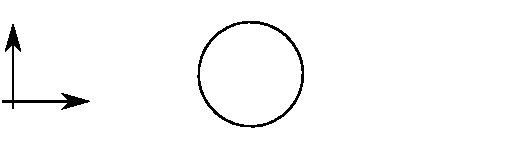
\includegraphics[width=\columnwidth]{figs/idealgrasp}
\caption{Cross-section from above showing an idealized two-finger (left) and three finger (right) gripper holding a cylinder.\label{fig:idealgrasp}.}
\end{figure}

While already very involved for anything but very simple mechanisms, such a model only captures a very small slice of realistic grasps. In any real application, contacts between a gripper and hand are not friction-less. This is the reason a grasp such as shown in Figure~\ref{fig:idealgrasp} actually works. If there were really no friction between the fingers and the object, the object would be ejected from the hand for every grasp that is not exactly aligned with a principal axis of the cylinder in Figure~\ref{fig:idealgrasp}, left. Furthermore, even the three-finger grasp shown in  Figure~\ref{fig:idealgrasp}, right, would \emph{always} fail as there is no force constraining the object from below. Fortunately, the existance of friction makes grasping much easier in practice, yet much harder to describe mathematically.

The reason that the grasps shown in Figure~\ref{fig:idealgrasp} do work in most circumstances is that the normal forces shown have a tangential component that is due to friction and covered by \emph{Coloumb's Friction law,}\index{Coloumb Friction}

which states that the higher the friction coefficient of a material, the more normal force translates into tangential forces that can resist two surfaces from moving against each other:

It is governed by the equation:
\begin{equation}
F_\mathrm{t} \leq \mu F_\mathrm{n}.
\end{equation}

Here $F_\mathrm{t}$  is the force of friction exerted by each surface on the other and $F_\mathrm{n}$ is the normal force. The force $F_\mathrm{t}$ acts in tangential direction of the normal force applied by, e.g., a finger's tip, where $\mu$ is an empirical coefficient of friction.

The friction coefficient $\mu$ is low for glass on glass and high for rubber on wood.  We are therefore interested in designing grippers with high friction coefficients to avoid objects from slipping.

When do objects slip? Lets say we have a fingertip pressing down on a surface in any orientation. There will be a force normal to the surface $F_\mathrm{n}$, which defines the tangential force $F_\mathrm{t}$ in any direction. Sweeping the tangential force around the normal force creates a cone with an opening angle of
\begin{equation}
\alpha=2tan^{-1}\mu,
\end{equation}
see \cite[p. 57]{rimon2019mechanics} for a derivation.
If the net force on the object is not within this cone, the object slips.  This becomes more intuitive when thinking about how different values of $\mu$ affect the shape of this cone. If $\mu$ is high, the cone will be relatively flat, letting the object accept forces from many different directions without slipping. If $\mu$ is low, the cone will be relatively narrow, requiring the force to be normal to the object's surface to prevent slippage.

\begin{figure}
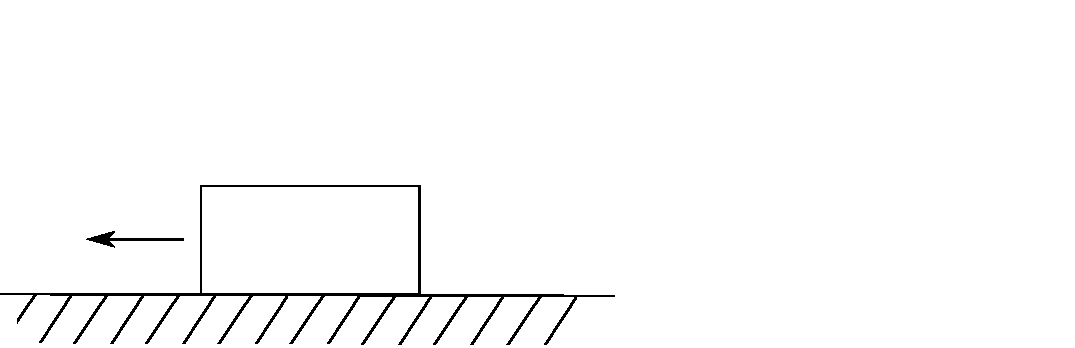
\includegraphics[width=\columnwidth]{figs/coulombfriction}
\caption{Left: Coloumb friction relates normal to tangential reaction forces that are required to overcome friction, here shown for rightwards motion. Right: Friction cone for point forces. As long as the force is within the cone cone, the finger will not slip.} 
\end{figure}

A force applied to a rigid body will exert both a force as well as a torque to the body's center of gravity. This is called a \emph{wrench}\index{Wrench}. If we consider the possible forces that we can apply to a rigid body without having the end-effector slip to form a space (namely the cone described earlier), we can talk about the \emph{grasping wrench space}\index{Grasping wrench space}, which is the corresponding space of all suitable wrenches.

Knowing the relation between normal and tangential reaction forces can help in designing grippers that are more likely to successfully grasp an object than others, as well as when planning suitable grasp for objects with known friction.

%In summary: we can use Coloumb's law of friction to determine the direction of forces that we can apply to a certain contact point without that the object slips. These forces translate into wrenches to the object's center of gravity. A grasp fits a certain task if the wrenches that would fulfill the task can be effectuated without slip. The less force is waisted to overcome slip, the better is the grasp.

\subsection{Multiple contacts and deformation}
In practice, no force will ever be applied at a single point only, but over an area, either due to the size of the finger pad itself or due to the contact area deforming. Even the smallest contact area will allow to not only additional force constraints, but also constraints on torque, thereby adding constraints in additional dimensions and therefore further stabilizing the grasp. This is illustrated in Figure~\ref{fig:contactarea}. Whereas the object can easily pivot around the point of contact in Figure~\ref{fig:contactarea}, left, increasing the area of contact constrains the rotational degree of freedom. It is therefore desirable to grasp an object with an as large contact area as possible. As surfaces are not ideally flat, in practice this is only possible when the contact area is deformable, Figure~\ref{fig:contactarea}, right. A large contact area will also increase friction.

\begin{figure}
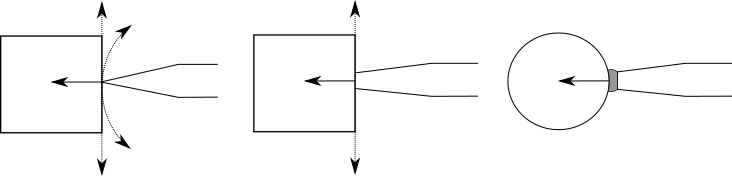
\includegraphics[width=\columnwidth]{figs/graspingcontacts}
\caption{From left to right: ideal force exerted via a single point of contact, forces exerted via an area of contact, contact area increasing due to pressure and conforming with the surface. Remaining degrees of freedom are indicated by dotted lines.\label{fig:contactarea}}
\end{figure}

Indeed, using blank metal grippers or fingers is little successful in practice. Instead, rubber pads are used to increase force closure by conforming around the object. As the rubber is flexible, however, the grasp is not completely fixating the object, but it can move within the grasp, which might not be desirable when picking up a nut, e.g., and trying to mount it on a screw. Mathematically, this introduces additional complications into the grasp model, as flexible pads are the equivalent of a spring, increasing uncertainty and dynamics. 

\subsection{Suction}

A highly capable method for grasping is using suction. Here, a suction cup is pressed against an object, using a vacuum applied by a pump to suck the object against the cup. Instead of exerting forces against the object, which always requires at least one antipodal force (or multiple forces that are distributed such that the object remains in equilibrium), suction only requires one point of contact. The rim of the suction cup provides both friction, to prevent the object from slipping, and multiple contact points that further constrain the object beyond the normal force applied by the vacuum. The soft nature of the suction cup provides the ability for the rim to conform to the object, making suction impractical for objects that do not have any flat surfaces. The elasticity of the rim also makes it difficult to further manipulate the object as all forces applied by the robot will need to be transferred via a spring-like elastic material.

\section{Simple grasping mechanisms}
Understanding why grasping actually works, namely due to friction and multiplying contacts by deformation, allows us to select grasping mechanism that are both able to successfully grasp a wide range of object and simple to construct. Here, properties of interest are the range of possible object sizes, given by a minimum and maximum size, the maximum weight of an object, and how fragile objects can possibly be. Here, object dimensions are directly dependent on the gripper kinematics, such as minimum and maximum aperture, whereas the maximum weight is given by the torque the mechanism can exert as well as the number of contacts and friction thereof. Whether a gripper can handle fragile objects is a function of how well this torque can be measured and controlled. 

\subsection{1-DoF scissor-like gripper}
One of the simplest grippers is a simple one degree-of-freedom claw, which is a popular design in the prosthetic community, and has been refined for centuries. Actuated by a string actuated by a person's shoulder or more recently by electric motors measuring muscle activity in the lower arm, this simple mechanism enables their wearers to perform a wide range of everyday activities. Indeed, an off-the-shelf prosthetic hand has been shown to perform a large variety of grasping and manipulation tasks, only limited by its ability to conform to specific kinematics such as operating scissors \cite{patel2016manipulation}.

\begin{figure}
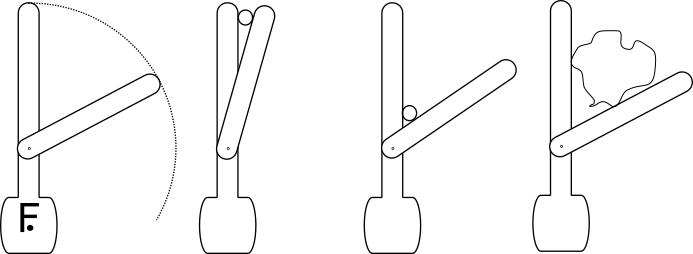
\includegraphics[width=\columnwidth]{figs/gripper-1-dof}
\caption{Simple 1-DoF grasping mechanism that relies on friction to grasp objects with a wide variety of sizes (center, right). The mechanism has only one moving part that presses the object against a passive finger. \label{fig:gripper-1-dof}}
\end{figure}

A simple design is shown in Figure~\ref{fig:gripper-1-dof} and consists of an active finger that presses an object against a passive finger, with both fingers often shaped as a hook. As should be clear by now, such a design can only work by relying on friction, which makes it not very common in traditional robotics. 

The key advantage of this mechanism is the very simple control strategy that it enables: use the passive finger to make contact with the object, then use the active finger to close the grasp. The event ``make contact" can either be detected by measuring the force at the wrist and looking for abrupt changes or using a tactile sensor on the surface with which contact is made. This approach can therefore lead to robust grasps with a minimum of sensing. A disadvantage of this mechanism is that its function relies exclusively on friction, possibly ejecting objects from its grasp if friction is not sufficient or the object is in an otherwise suboptimal conformation. Unlike most other mechanisms, it is also impossible to use the finger position to infer the width of an object, which is illustrated by the illustrations in Figure~\ref{fig:gripper-1-dof}, center. 

The mechanism shown in Figure~\ref{fig:gripper-1-dof} can be actuated in many different ways, for example by attaching a servo motor directly to the active finger, using a shape-memory alloy wire via a suitable lever arm, or a pneumatic piston or balloon.

\subsection{Parallel jaw}
The most common industrial mechanism is the two-finger parallel jaw gripper. It operates by squeezing an object between its two parallel fingers, which are usually driven by a single actuator and thereby move in concert. Although it also relies on friction, parallel fingers usually yield more contact area than a scissor-like 1-DoF gripper, but suffers from a smaller range of motion. 

\begin{figure}
\centering
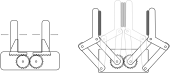
\includegraphics[width=\columnwidth]{figs/gripper-2-dof}
\caption{Left: Parallel jaw gripper driven by a single actuator via a system of coupled gears.Right: 4-bar linkage parallel jaw gripper. \label{fig:paralleljaw}}
\end{figure}


Figure~\ref{fig:paralleljaw}, left, shows a minimalist implementation of a parallel jaw gripper that can be actuated by a single servo motor, driving two rack gears to which the gripper jaws are mounted. While using gears and rack gears is unusual --- the gripper jaws typically travel on threads actuated by worm gears or are attached to a pneumatic piston --- this drawing illustrates the relationship between the range of motion of the gripper jaws, the length of the mechanism it is sliding on, here a rack gear, and the resulting body size. In order for this design to fully close, the two rack gears must be mounted at an offset. These constraints often make the gripper body twice as wide as the maximum aperture, making it difficult for the robot to enter tight areas. The mechanical design also affects the speed at which a gripper can operate. Pneumatic grippers, where air pressure coming in on either end of the piston can drive the gripper into an ``open'' or ``close'' position very quickly (2-3 times per second), but cannot be controlle accurately. Electric mechanisms instead trade accuracy and torque with speed as the jaws move on a thread or racket gear. 

The control strategy for parallel jaw grippers requires an accurate pose estimate of the object of interest and positioning the gripper so that the object is right in the center of the two jaws. Note that force-closure with a static object, such as a screw mounted to a structure, requires both jaws to make contact with the object, thereby imposing high accuracy requirements of both object detection and robot motion. Here, compliance can help, allowing the gripper to adjust its pose to the object. This can be accomplished by either measuring forces in the wrist and moving the gripper to minimize lateral forces or a compliant mounting mechanism or structure, such as a robot equipped with series-elastic or pneumatic actuators. An alternative approach is to actuate both gripper jaws independently.


\subsection{4-bar linkage parallel gripper}
A parallel jaw mechanism with a larger range of motion can be accomplished using two 4-bar linkages, Figure~\ref{fig:paralleljaw}, right. In a 4-bar linkage, rotation is translated into  straight translation. This is accomplished by two pairs of parallel bars of equal lengths. In Figure~\ref{fig:paralleljaw}, right, one of the four bars is not moving and substituted by the gripper body, to which two of the bars are mounted. Interestingly, both pairs remain parallel as one of the bars is rotating, resulting in the two gripper jaws remaining parallel to each other. This is best understood by inspecting Figure~\ref{fig:paralleljaw} and comparing the two positions the left jaw can be in. 


The drawback of this design is that closing the gripper also results in a forward motion. This requires approaching an object from different heights, depending on its width. Other than this, the control strategy is the same as for the parallel jaw gripper, requiring an accurate estimate of the object's pose. Also here, adding compliance or independent actuation can help resolving accuracy problems. 

\subsection{Multi-fingered hands}
There are rarely used more than two fingers/jaws in industrial practice. One common use case is grasping cylindrical objects from above, for which three fingered hands, such as indicated in Figure~\ref{fig:idealgrasp}, right, are best suited. In most other cases, three fingers are not an advantage, and might even a hindrance. This has led to designs in which two of the fingers are reconfigurable from performing an inwards motion to behave identical to a parallel jaw gripper, while the third finger is stored in a safe position. 

How many grasps are possible and how many possible grasps are needed to grasp every possible object remains a difficult theoretical problem (which is further complicated by the fact that successful grasping often happens at the boundary of what is mathematically tractable). Generally, we can say however, that additional fingers --- such as in the human hand --- provide additional redundancy, which allows grasping and manipulating (see Section \ref{sec:manipulation}) the same object in many different ways, including manipulating the object within the hand, that is without intermettent placement or handing it over to another gripper. 

%\section{What is a good grasp?}
%We can also define wrench spaces that suit a specific task, such as picking up an object or opening a door by turning its knob. We can then say that the grasp is ``good'', when the task wrench space is a subset of the grasping wrench space, and will fail otherwise. We can also look at the ratio of forces actually applied to the object and the minimum needed to perform a desired wrench. If this ratio is high, for example, when the robot has to squeeze an object heavily to prevent it from slipping, this grasp is not as good as one, where the ratio is low and all of the force the robot is exerting is actually going into the desired wrench.


\section{How to find good grasps?}

It is usually not possible to find close-form expressions for the grasping wrench space. Instead, one can sample the space of suitable force vectors, e.g., by picking a couple of forces that are on the boundary of the cone's base, and calculate the convex hull over the resulting wrenches.



We are able to determine whether a contact point leads to a good grasp by comparing the grasping wrench spaces that fulfill the task and those that is created by a set of contact points. The question is now how to find good contact points? This is challenging as end-effectors (such as hands) are already quite complicated. A suitable method is therefore to use random sampling, that is bringing the end-effector to random positions, close its fingers around the object, and see what happens when generating wrenches that fulfill the task's requirements.

To close the end-effector's fingers around the object requires collision checking. To see what happens, requires dynamic simulation. In short, collision checking routines model an object using a mesh of triangles that can be generated using CAD tools. These triangles are the leafs of a tree that has a coarse bounding object at the top. This coarse bounding object is then split into smaller and smaller elements. Collision checking can now quickly test whether an object collides at all and then recursively refine the exact triangles that collide and finally find the exact points of collision. Dynamic simulation applies Newtonian mechanics to an object (i.e., forces lead to acceleration of a body) and moves the object at very small time-steps. Detecting a collision usually involves moving the objects one step back and then iteratively approaching them until their proximity exceeds a certain treshold.

\section{Manipulation}\label{sec:manipulation}
While grasping is only concerned with attaching an object to a robot's kinematic chain, it is often the case that such an object is not just placed or dropped, but that the intention of the grasping action was to change the pose of this object in some meaningful way. For example, cutlery and dishes on a table need to be in well-specified areas and aligned with each other, merchandise needs to be neatly stacked in a shelf, and machine parts need to be assembled with each other. These activities are known as \emph{manipulation}. Discussing all the possible ways objects might be manipulated, for example inserted, screwed-in, turned, twisted, flipped, etc., and the many different contexts such actions would be required --- which might dramatically change the approach a robot would need to chose --- are well beyond the scope of this book.

Yet, many manipulation problems can be cast into a sequence of grasping and placing problems in which the possible grasp choices are appropriately constrained. For example, an object can be turned or flipped by planning a sequence of pick-and-place movements that each turn the object by a certain degree. Similarly, using two robotic arms, with one grasping an object out of the hand of the other, will allow a robot system to change an object's pose almost arbitrarly. (Which poses an object will be able to reach will depend on the object's exact geometry, the kinematics of the robotic arms, and constraints in the workspace.) So-called \emph{in-hand manipulation}\index{In-hand manipulation} is still an active area of research as  repeatedly picking and placing an object and hand-overs between different arms is considered to be too slow and otherwise impractical for many application areas.  

\subsection{Peg-in-hole problems}
\subsection{Non-prehensile Manipulation}

\section{Exercises}
\begin{enumerate}
\item Think about at least three mechanisms to realize a parallel jaw gripper. How does the minimum and maximum aperture of the gripper relate to the gripper width for each of these designs?
\item Think about at least three mechanisms to actuate a four-bar linkage. Which of these will keep the payload inside the gripper during power failure?
\item Derive an equation for the distance of the fingertip from the gripper base in a 4-bar linkage gripper as a function of the gripper opening width. Use appropriate parameters for all unknown parameters. 
\item Write code to generate rectangles with random dimensions and orientations. Use a point-in-polygon test to simulate random samples on its surface. Apply principal component analysis to compute the principal axes of the rectangle and compare with ground truth. How does the number of samples affect the accuracy of your estimate?
\end{enumerate}
